\usubsection{Caso 3}

\usubsubsection{Solución Teórica}

\begin{align*}
  R&=5k\Omega&
  C&=470\mu F&
  L&=5mH
\end{align*}
En este caso $t_0=0$.
\begin{align*}
  s_1 &= \frac{-\frac{5k\Omega}{5mH}
  - \sqrt{\left(\frac{5k\Omega}{5mH}\right)^2-\frac{4}{5mH470\mu F}}}{2}
  &
  s_2 &= \frac{-\frac{5k\Omega}{5mH}
  + \sqrt{\left(\frac{5k\Omega}{5mH}\right)^2-\frac{4}{5mH470\mu F}}}{2}
\end{align*}

\usubsubsection{Simulación}

\begin{figure}[H]
  \begin{lstlisting}
    model RLCSerie3
      import Modelica.SIunits.Resistance;
      import Modelica.SIunits.Capacitance;
      import Modelica.SIunits.Inductance;
      import Modelica.SIunits.Voltage;
      import Modelica.SIunits.Current;

      parameter Resistance R = 5000.0;
      parameter Capacitance C = 0.000470;
      parameter Inductance L = 0.005;

      Voltage Vs, Vr, Vl;
      Voltage Vc(start=0, fixed=true);
      Current Il(start=0, fixed=true);

    equation
      Vs = if (time >= 5.0 and time <= 7.0) or (time >= 15) then 10 else 0;
      Vr = R * Il;
      Vl = L * der(Il);
      Il = C * der(Vc);
      Vs = Vr + Vl + Vc;
      annotation(experiment(StartTime=0.0, StopTime=25.0));
    end RLCSerie3;
  \end{lstlisting}
  \caption{Código para el tercer caso.}
\end{figure}

\begin{figure}[H]
  \centering
  \label{gr:caso1:corrientes}
  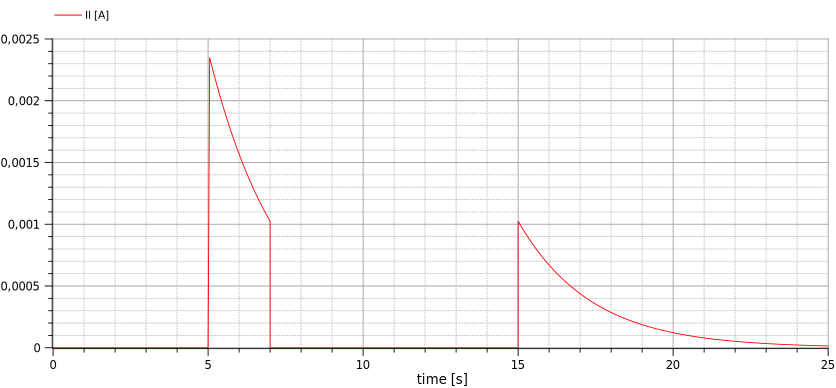
\includegraphics[width=\textwidth]{modelica/graficas/3-corrientes}
  \caption{Gráfica de Corrientes para el tercer caso.}
\end{figure}

\begin{figure}[H]
  \centering
  \label{gr:caso1:tensiones}
  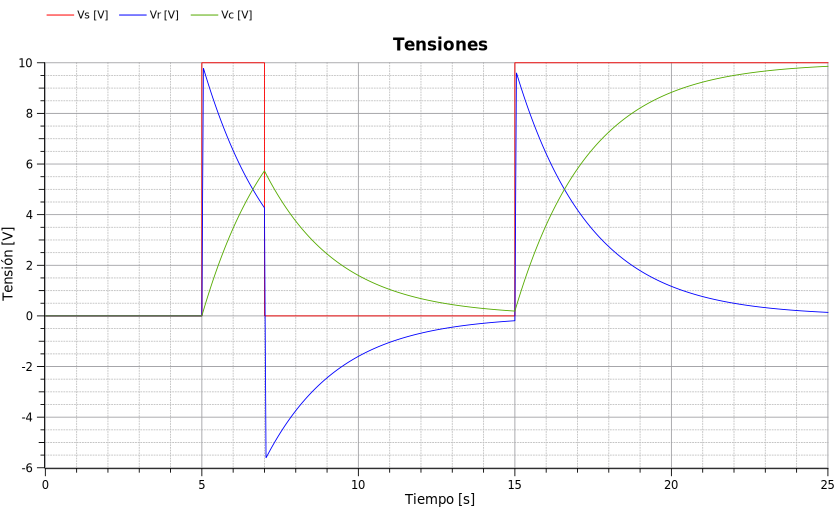
\includegraphics[width=\textwidth]{modelica/graficas/3-tensiones}
  \caption{Gráfica de Tensiones para el tercer caso.}
\end{figure}
